%tipos de codigos qr
\section{Tipos de Códigos QR}

\subsection{Código QR Modelos}
\begin{figure} 
	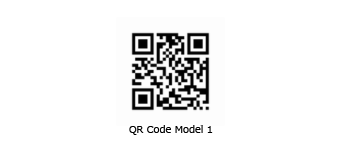
\includegraphics[width=0.4\linewidth]{model1Image.png}
	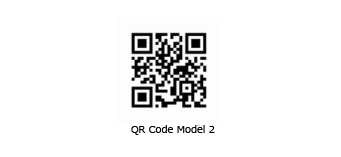
\includegraphics[width=0.4\linewidth]{model2Image.png}
	\label{fig:QRModels}
\end{figure}

\subsubsection{Código QR Modelo 1}
Es el código QR original, es capaz de codificar 1,167 números con una versión máxima de 14 (73 x 73 módulos). \cite{qrcode2021}

\subsubsection{Código QR Modelo 2}
Mejora del modelo 1 para que este código se pueda leer sin problemas incluso si está distorsionado de alguna manera. Por ejemplo, si los códigos QR están impresos en una superficie curva o distorsionada de alguna manera, debido al ángulo de lectura se pueden leer de manera eficiente, utilizando sus patrones de alineación. Estos pueden códificar 7,089 números, siendo su versión máxima de 40 (177 x 177 módulos).\cite{qrcode2021}

\begin{figure} 
	\centering
	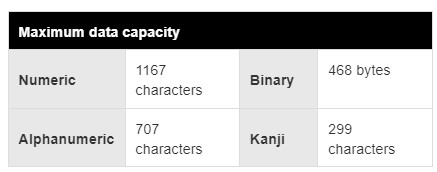
\includegraphics[width=0.7\linewidth]{qrmodel1Maxdata.jpg}
	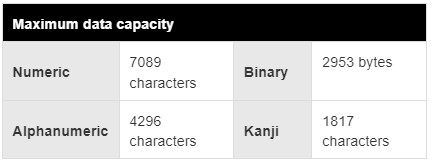
\includegraphics[width=0.7\linewidth]{qrmodel2Maxdata.jpg}
	\caption{Capacidad Máxima de datos del modelo 1 y 2 respectivamente.}
	\label{fig:qrmodel2Maxdata}
\end{figure} 

\subsection{Micro código QR}

En 1998, se desarrolló el micro código QR que mantiene el rendimiento de lectura del código QR, permite la codificación de 20 caracteres alfanuméricos que se incluían en códigos de productos y número de series, siendo impreso en un cuadrado de 1mm.\cite{2019_Hara}
\begin{figure} 
	\centering
	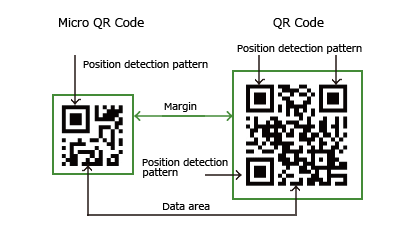
\includegraphics[width=0.4\linewidth]{microQrImage.png}
	\caption{Diferencias entre un código QR y uno micro código QR.}
	\label{fig:microQR}
\end{figure}
El micro código QR se distingue por el hecho de que solo tiene un patrón de detección de posición, en comparación con el código QR que requiere un área, dado que los tres patrones de detección de posición se encuentran en las esquinas del símbolo. Mientras que el micro código QR solo requiere un margen de dos módulos alrededor de un símbolo, donde el Código QR tradicional requiere al menos un margen de cuatro módulos. Esto permite que sea impreso en áreas incluso más pequeñas que el código QR. La cantidad máxima de datos que puede almacenar es de 35 números, con una versión máxima M4 (17 x 17 módulos).\cite{qrcode2021}



\subsection{Código iQR}
El código iQR es un código bidimensional que permite una fácil lectura de su posición y tamaño. Tiene una amplia gama de códigos de tamaño, puede contener una mayor cantidad de datos que el código QR tradicional, con el mismo tamaño se puede contener un 80\% más que este último. Además, el código iQR es de 9 x 9 módulos con eso se puede reducir un 30\% más pequeño en relación a el código QR que consta de 11 x 11 módulos. Este código se puede imprimir como un código rectangular, un código invertido, inversion de los colores de los módulos o un código de patrón de puntos (marcado directo de piezas). Debido a esto, es posible colocarlos en una superficie cilíndricas manteniendo su legibilidad del código, lo que no es posible con códigos cuadrados.\cite{qrcode2021}
\begin{figure} 
	\centering
	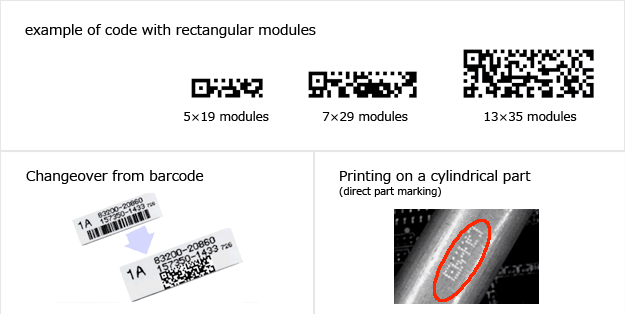
\includegraphics[width=0.8\linewidth]{iQrFeature3Image.png}
	\label{fig:iqr}
\end{figure}
\begin{figure} 
	\centering
	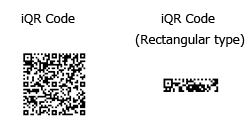
\includegraphics[width=0.4\linewidth]{iQrCodeImage.png}
	\caption{Código Cuadrado y Código Rectangular, respectivamente.}
	\label{fig:iqr2}
\end{figure}

Por otro lado, el número de caracteres que puede almacenar el código iQR es de 40,000 caracteres numéricos en su versión más grande (422 x 422 módulos). En donde su nivel de corrección de errores es de hasta el 50 \%. Su forma rectangular, el mínimo es de 5x19 puede almacenar 6 números y el de módulo máximo es de 43 x 131, aproximadamente 1,200 caracteres.\cite{qrcode2021}
El código iQR rectangular con mayor eficiencia de datos fue desarrollado en 2008.\cite{2019_Hara}

\subsection{Código SQRC}
Utilizando la tecnología Secure QR Code (SQRC) para mantener la información segura y oculta. Debe señalarse que para compartir la información personal confidencial es necesario la validación y autorización del código QR mediante el algoritmo criptográfico de clave pública RSA.\cite{Ahamed2019}
La estructura del código SQRC cuenta con dos capas, una región de información abierta y una región de información cerrada. La región abierta puede ser leída por cualquier dispositivo con capacidad de escaneo, mientras que la region cerrada encryptada que solo se puede leer con dispositivos que cuenten con las claves de cifrado coincidentes y un software especial de reconocimiento (para verificar que los datos no sufrieron alteraciones).\cite{2019_Hara}
\begin{figure} 
	\centering
	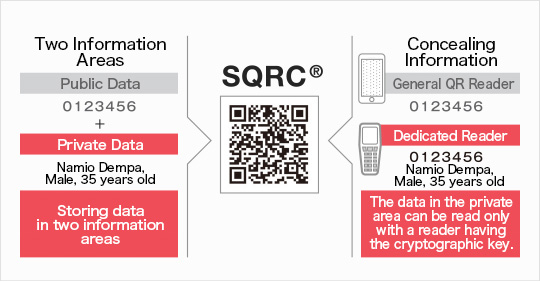
\includegraphics[width=0.4\linewidth]{SQRC.jpg}
	\caption{Utilizando una clave criptográfica para mantener la información privada y con esto restringir los tipos de dispositivos que pueden leer la información.}
\label{fig:sqrc}
\end{figure} 

El código SQRC puede evitar la falsificación y manipulación. El código QR aunque tiene mayor espacio y gran capacidad, se puede leer la información con cualquier dispositivo, incluida la información privada y clasificada, por esta razón no es seguro. El uso de este código puede darse en Hospitales (protección y gestión de información personal), Delivery de albaránes entre empresas, instalaciones de eventos y parques de atraciones.\cite{qrcode2021}

\subsection{Código Frame QR}
Frame QR es un código con la misma capacidad que el código QR original, pero establece un lienzo especial que contiene algún logotipo o imagen en el centro del código. \cite{2019_Hara}
\begin{figure} 
	\centering
	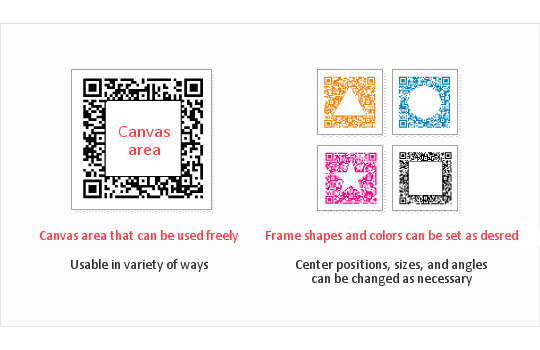
\includegraphics[width=0.6\linewidth]{FrameQR.jpg}
	\caption{Tiene un área que puede contener un tipo de forma, logotipo o imagen dentro de ella.}
	\label{fig:frameqr}
\end{figure}
Este código tiene un marco para contener una imagen. Tanto la forma del marco y el color se pueden cambiar, se puede aplicar a una variedad de aplicaciones. El uso de este código puede darse en Tarjetas de visita y catálogos, Medidas anti-falsificación y trazabilidad.\cite{qrcode2021}